\documentclass[../sherrill-Mix_thesis.tex]{subfiles}
\begin{document}
\chapter{Conclusions and future directions}
\graphicspath{{im/}{conclusion/im/}}

In this dissertation, we described studies to characterize the nature of HIV-1 latency, characterize expression and alternative splicing and host cell response to infection and develop alternative methods for detection of infection and quantification of viral loads.

A common theme was that cell lines and \textit{in vitro} models of these replication steps often disagree with each other and with primary cell data. 

\section{Latency and integration location}

	In Chapter \ref{chapLatency}, we showed that the chromosomal location of integration affects proviral latency but the mechanisms appear to differ between cell culture models. Similarly a recent study of nine cell culture models found that no single model reliably predicted the performance of activating compounds in \textit{ex vivo} tests of latently infected cells from HIV patients \citep{Spina2013}. This suggests that either some cell culture models do not accurately reflect latency in patients or that there are diverse subsets of cells with differing mechanisms of latency within patients. 

	Cell culture models are currently used to screen potentially therapeutic compounds \citep{Xing2011,Spina2013}. If some cell culture models are not representative of \textit{in vivo} conditions then potential treatments may be discarded or marked for development erroneously. Further comparisons between additional cell culture models and additional replicates of existing models might allow discrimination between batch/lab effects and reveal patterns between models. Comparison with cells extracted from patients or infected lab animals might offer a gold standard comparison although it is difficult to obtain large amounts of cells and difficult to distinguish defective provirus from latent provirus in such populations. %Perhaps cell sorting for a marker of viral activity, applying a strong inducing agent and sorting again for newly expressed virus.

	Various treatments are now being considered for the reactivation of latent provirus \citep{Spina2013}. To further understand the mechanisms of these treatments, it would be informative to compare the features of latent provirus induced by a given treatment to latent viable provirus remaining uninduced. Repeated cell sorting and integration site sequencing might provide insight on mechanism. For example, one could first sort out cells with active provirus, then treat with the potential latency modulator and sort out cells with newly active provirus and then treat with a strong inducer or alternative stimuli and sort out cell with newly activated provirus. This would give subsets of cells where latent proviruses had been activated by treatment and cells with provirus which were not activated by treatment but still inducible. Synergies between treatments could be assessed and the location of integration sites could be determined and used to locate patterns of genomic features correlated with induction for each treatment.

	Current efforts at ``shock and kill'' therapy, inducing latent virus to activate and eliminating infected cells, focus on histone deacetylase inhibitors. If there are diverse mechanisms of latency within patients then much of the latent reservoir may remain unactivated by single target therapies.  Clinical trials with histone deacetylase inhibitors have shown some small increases in viral RNA but little decrease in the latent reservoir of HIV \citep{Lehrman2005,Archin2010,Archin2012,Spivak2014}. It appears that the majority of viable latent provirus from patient cells are not reactivated by current therapies \citep{Cillo2014}. These results are particularly worrisome since 10,000-fold or more reductions of the latent reservoir are likely to be necessary to functionally cure HIV \citep{Hill2014}.

	In Chapter \ref{chapLatency}, we used publicly available genomic data. Perhaps there is some chromosomal feature with a strong association with latency but the data is not currently available or varies greatly between cell populations. More varieties of annotations are rapidly becoming available \citep{ENCODEPC2012,Barrett2013,Karolchik2014,Goldman2015,Cunningham2015}. Decreasing sequencing costs \citep{Metzker2010,Mardis2011,Wetterstrand2015} may also make it feasible to measure more epigenetic features in the exact cell population of interest. Repeating analysis similar to Chapter \ref{chapLatency}, perhaps by simply rerunning the reproducible report in Appendix \ref{appLatencyReport}, with new data would allow any new features to be monitored for correlations with latency.



\section{HIV-1 alternative splicing}
	In Chapters \ref{chapPacBio} and \ref{chapRnaSeq}, we showed that HIV RNA spliceforms are more diverse than previously appreciated and estimated the abundances of viral spliceforms. We also showed that splicing at some splice sites vary between host subjects, between cell types and over the course of infection. Further characterization of viral splicing would be beneficial to the study and treatment of HIV-1 especially as there were some technical limitations to our research that might be improved upon using current techniques.
	
	We studied HIV splicing using droplet PCR \citep{Tewhey2009} and a set of customized primer in Chapter \ref{chapPacBio} and bulk sequencing of cellular mRNA in Chapter \ref{chapRnaSeq}. Sequencing biases and difficulties determining full length transcripts from short reads hindered characterization of HIV sequencing. One alternative to these techniques is the targeted capture and enrichment \citep{Depledge2011,Mercer2014} of HIV-specific sequences. Using probes targeted to conserved regions of HIV, similar to the work in Chapter \ref{chapLamp}, would allow for enrichment of viral reads without the biases induced by primer-based PCR while still allowing for efficient use of sequencing effort.

	The research in Chapter \ref{chapPacBio} was also limited by a short read bias in the PacBio sequencing. PacBio sequencing has improved \citep{Mosher2014} and additional long read sequencers have been developed \citep{Mikheyev2014,Jain2015,Kilianski2015}. In addition, Illumina MiSeq sequencers can now produce 25 million paired 300 bp reads in a single run \citep{Juenemann2013,Illumina2015} and better spliceform estimation methods are being developed \citep{Rossel2014,Bray2015}. These improved sequencing techniques might allow for more straightforward analysis of new samples and verification of our previous results.

	Transcripts transcribed antisense to the canonically expressed strand of HIV have been observed \citep{Michael1994,Landry2007,Lefebvre2011,Schopman2012,Kobayashi-Ishihara2012,Saayman2014}. These transcripts may be translated to proteins \citep{Ludwig2006,Toresilla2013} that trigger immune response in infected individuals \citep{Ludwig2006,Bansal2010}.  Our sequencing techniques were designed only for the HIV positive strand (Chapter \ref{chapPacBio}) or did not preserve strand information (Chapter \ref{chapRnaSeq}). Strand-specific sequencing \citep{Levin2010,Podnar2014} of various HIV strains under varying cellular conditions would help to clarify the identity of these transcripts. Ribosome profiling \citep{Ingolia2009,Ingolia2011,Ingolia2014} of infected cells might also clarify whether these transcripts are likely to be translated. These cryptic transcripts could offer a new opportunity in vaccine design \citep{Bansal2010} but first their abundance, identity and conservation across strains of HIV must be ascertained.
	
	 We observed that splicing varies over the course of infection, between human subjects and between cell types. Further sampling would help to clarify patterns in these splicing changes. [[A sentence on macrophage and resting]] [[long term non progressors]] [[24 hour in life HIV]] [[]] Additional cell types, in particular macrophage \citep{Carter2006},  [[many previous studies in lab strains]] [[more patient strains]] [[founder virus]] [[other retrovirus]]
	 %In addition to the improvement sequencing techniques, the cost of sequencing is dropping \citep{Metzker2010,Mardis2011,Wetterstrand2015}.

	Disruption of RNA processing can drastically viral replication \citep{Wetz1997,Caputi2004,Madsen2005,Paca-Uccaralertkun2006,Mandal2008}. Small molecules that inhibit cellular SR splicing proteins and disrupt viral splicing show promise as antiretroviral therapies \citep{Fukuhara2006,Bakkour2007,Wong2011,Wong2013}. A better understanding of viral splicing may lead to better treatment.

	




Further clarification using more detailed sequencing in more time points, cell types and strains of HIV-1 and other lentiviruses rema

PacBio was bad. Figure? Do better

In addition an important subset of HIV are the founder viruses transmitted between hosts \citep{Keele2008,Salazar-Gonzalez2009}. These viruses are not well studied and perhaps their splicing and gene expression differ from the rest of the viral swarm of late-term patients.

Evolution of new proteins and epitopes


\section{Host expression during HIV infection}

In Chapter \ref{chapPacBio}, we showed that HIV RNA spliceforms are more diverse than previously appreciated. We also showed that splicing varies between host subjects, between cell types and over the course of infection.

Differences in miRNA expression between infected and uninfected and elite controllers and viremic patients by NanoString array but confounded by changes in proportion of \cdFour T cells\citep{Witwer2012}. Poor cell culture characterization with SAGE-Seq, saw antisense HIV \citep{Lefebvre2011}. Illumina sequencing over time of infection, widespread changes (RNA extraction with mirvana kit)  \citep{Chang2011}.  Solid sequencing of short RNA in infection finds mostly positive strand miRNA and <2\% antisense possible miRNA and changes in tRNA Lys3\citep{Schopman2012}.

Recent research has shown that

miRNA http://jcs.biologists.org/content/128/8/1607.full 

Small RNA sequencing would also allow further characterization of viral small RNAs. Viral derived microRNA, perhaps in part from Dicer processing of the structured trans-activation response element structured RNA of HIV \citep{Klase2007,Oullet2008,Schopman2012,Klase2009}, may suppress HIV expression \citep{Omoto2004,Triboulet2007,Chable-Bessia2009} and inhibit apoptosis \citep{Klase2009} but the presence of such miRNA is controversial \citep{Pfeffer2005,Lin2007}. HIV may suppress miRNA silencing \citep{Bennasser2005,Triboulet2007,Qian2009} but controversial \citep{Lin2007}

%http://www.lifetechnologies.com/us/en/home/life-science/dna-rna-purification-analysis/rna-extraction/rna-types/total-rna-extraction/magmax-technology.html

Non polyadenylated RNA Katze paper. Strand specific sequencing. Longer reads and longer fragments.

Localization nucleus vs cytoplasm

Cell types, macrophages

Infection, sorting

Cell lines bad

Endogenous retrovirus

intron retention

viral proteins

immune response

\section{LAMP PCR and lab-on-a-chip}
		In Chapter \ref{chapLamp}, we report a loop mediated isothermal amplification system using primers optimized to to detect most subtypes of HIV-1. An alternative to a single broadly targeted primer set would be to design separate primer sets targeted specifically to each subtype so that a positive amplification would then be able to discriminate viral subtype. Different viral subtypes can have different rates of disease progression \citep{Kanki1999,Kaleebu2002,Baeten2007,Kiwanuka2008}, transmission dynamics \citep{Renjifo2004,John-Stewart2005,Huang2007b} and response to treatment \citep{Snoeck2006,Easterbrook2010,Scherrer2011}. Simple low-cost devices with multiple reactions chambers could be used to both identify viral subtype and estimate viral load \citep{Liu2014a,Mauk2015} and allow modified treatment decisions.
		
		A LAMP chip with subtype-specific primers would also allow the detection of some superinfections. Superinfection of a single individual with multiple distinct strains of HIV is common in high risk individuals \citep{Piantadosi2007,Powell2009,Ronen2013,Wagner2013,Redd2014} and the general population \citep{Redd2012a}. Superinfection can lead to disease progression \citep{Jost2002,Fang2004,Blick2007,Gottlieb2007,Streeck2008,Clerc2010} or drug resistance \citep{Smith2005}. Superinfection also allows recombination between divergent strains \citep{Fang2004,Pernas2006,Blick2007,Piantadosi2007,Streeck2008} and this rapid exchange of genetic information can lead to more fit recombinant strains and worsen the global epidemic \citep{Robertson1995,Gao1999,Hahn2000,Malim2001,Blick2007}. LAMP detection of superinfection could allow early intervention and suppression in superinfected individuals.

		The techniques described in Chapter \ref{chapLamp} also allow for rapid development of detection assays for novel pathogens. For example, in a recent outbreak in West Africa, Zaire ebolavirus has infected over 26,000 confirmed, probable and suspected cases and caused over 11,000 reported deaths \citep{Gire2014,WHOERT2014,WHO2015}. Early detection and quarantine are essential to the control of this epidemic \citep{Chowell2014}. Amplification of Ebola virus nucleic acid through polymerase chain reaction is the best diagnostic test currently available but the necessary resources are often not available in these resource-poor regions \citep{Fauci2014,WHO2015a}. Antigen-based tests are quicker and available at the point-of-care but are not as accurate or sensitive as polymerase chain reaction tests and are still in limited supply \citep{WHO2015a}.  Loop-mediated isothermal amplification offers the potential for rapid, sensitive and efficient detection of Ebola RNA but currently available LAMP primers \citep{Kurosaki2007} do not match the outbreak strain. Using sequences from the recent outbreak \citep{Gire2014,Hoenen2015} and the methods described in Chapter \ref{chapLamp}, we designed primers to match all known Zaire ebolavirus \ref{figEbolaConsensus}. These primer combined with simple lab-on-a-chip devices for purifying blood plasma \citep{Liu2013} and imaging fluorescent signals \citep{Liu2011,Liu2014a} could allow rapid point-of-care detection of Ebolavirus.

	\begin{figure}
		\centering
		%%[[FIX THIS FIGURE and name Ebola right]]
		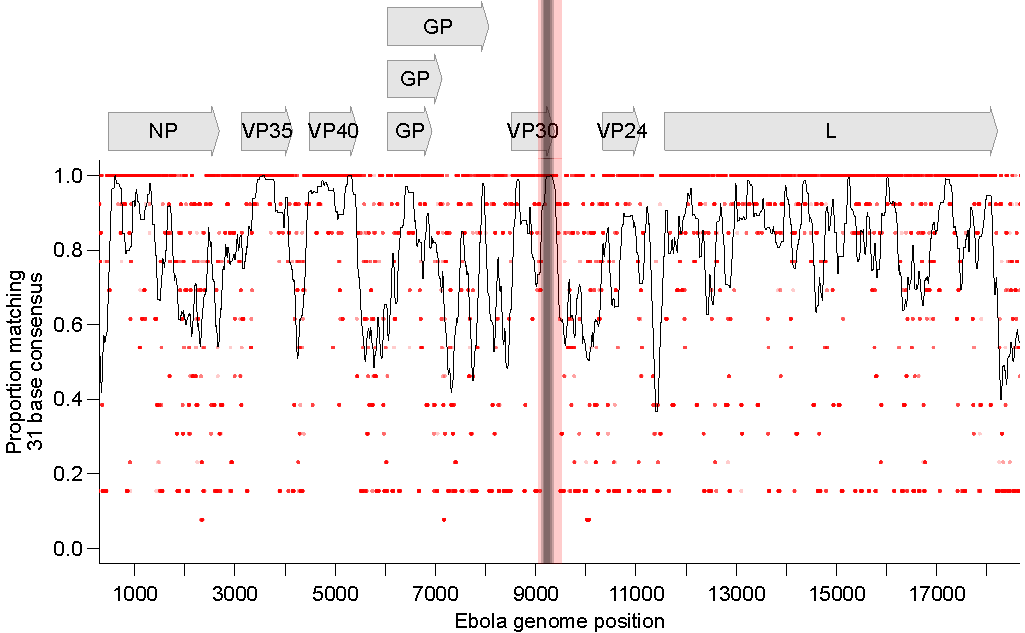
\includegraphics[width=.6\textwidth]{ebolaConsensus.pdf} %REMOVE%
		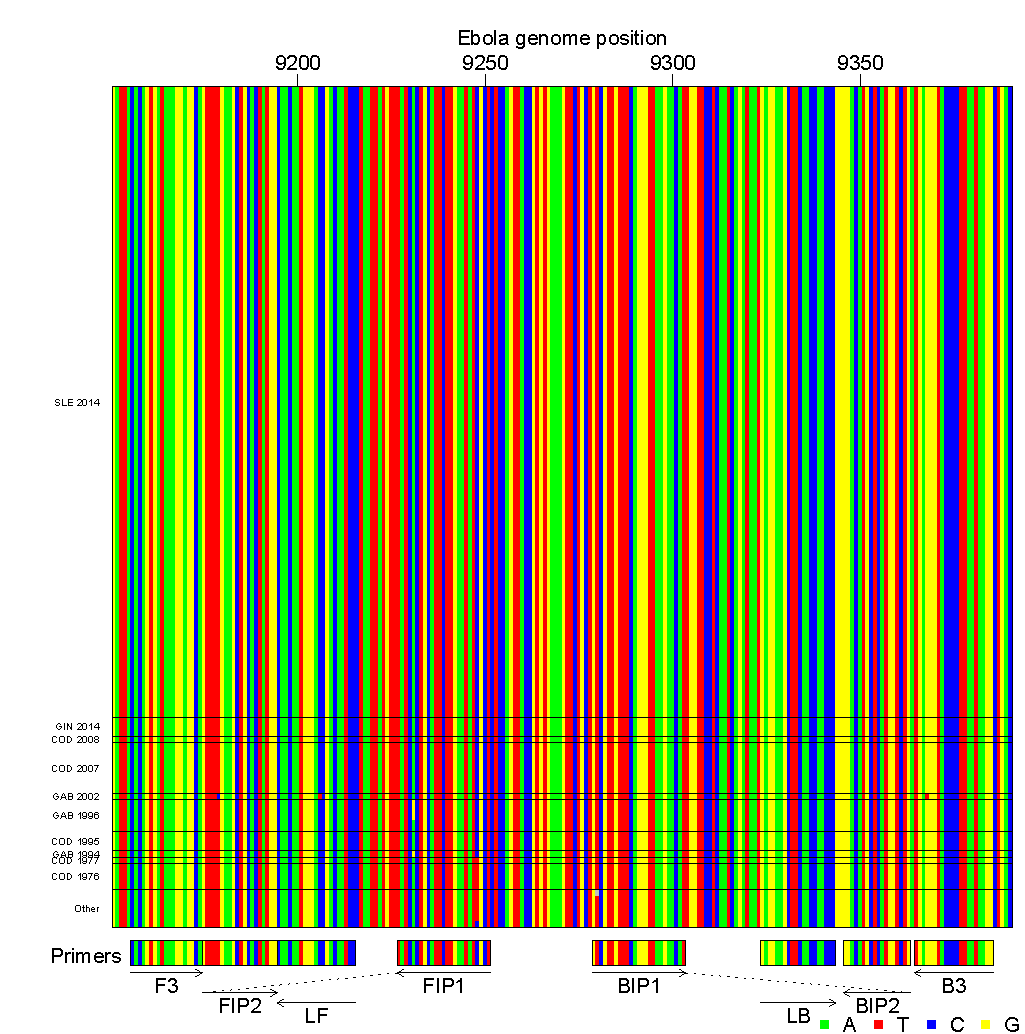
\includegraphics[width=.6\textwidth]{loop_bases.pdf} %REMOVE%
		\caption[Ebola RT-LAMP primers design]{Bioinformatic analysis to design Ebola RT-LAMP primers. A) Conservation of sequence in Ebola. Ebola genomes (n = 131) from Genbank and sequences from the recent Zaire Ebolavirus outbreak \citep{Gire2014} were aligned and conservation calculated. The x-axis shows the coordinate on the Ebola genome, the y-axis shows the proportion of sequences matching the consensus for each 21 base segment of the genome (red points). The black line shows a 101 base sliding average over these proportions. The vertical red shading shows the region targeted for LAMP primer design that was used as input into the EIKEN primer design tool. Numbering is relative to the Ebola Mayinga sequence. B) Aligned genomes, showing the locations of the preliminary primers. Sequences in the red shaded region in A are shown, with DNA bases color-coded as shown at the lower right. Each row indicates an HIV sequence and each column a base in that sequence. Horizontal lines separate Ebolavirus outbreaks (labeled at left). Arrows indicate the strand targeted by each primer. Primers targeting the negative strand of the virus are shown as reverse compliments for ease of viewing.}
		\label{figEbolaConsensus}
	\end{figure}

\subsection{Conclusions}
	These studies contribute to the study and treatment of HIV-1 by revealing aspects of latency, expression and host response. They highlight the importance of primary cell models and the effects that host cell can have on viral processes. With rapidly increasing sequencing throughput, studies like those presented in this thesis offer the opportunity for a deeper and broader understanding of HIV-1 biology and host response and further development of diagnostics and therapeutics.

\end{document}
